\chapter{Pianificazione}\label{Pianificazione}
Il gruppo \textit{Jawa Druids} ha pianificato le attività di progetto seguendo le scadenze riportate nel \S~\ref{IntroduzioneScadenze}}. Il progetto è dunque suddiviso nelle seguenti fasi:
\begin{itemize}
	\item Analisi;
	\item Consolidamento dei requisiti$_{\scaleto{G}{3pt}}$;
	\item Progettazione architetturale;
	\item Progettazione di dettaglio e codifica;
	\item Validazione e collaudo.
\end{itemize}
Ognuna di queste fasi è formata da attività$_{\scaleto{G}{3pt}}$ illustrate nei diagrammi di Gantt$_G$, che permettono la rappresentazione grafica di un calendario, utile al fine di pianificare, coordinare e tracciare specifiche attività dando una chiara illustrazione del suo stato di avanzamento.
Queste fasi hanno una durata media che varia da uno a due mesi e siccome questo può creare delle difficoltà sia nella fase di preventivazione sia nel tenere traccia dell'effettivo avanzamento del lavoro, il gruppo ha deciso di dividerle in sotto-periodi di tempo più brevi.
Per ognuno di questi sotto-periodi sono elencate le attività specifiche da svolgere, inoltre per le fase di Progettazione di dettaglio e codifica e per la fase di Validazione e collaudo tali attività sono specificate anche dagli incrementi individuati, dando un livello di pianificazione ancora più dettagliato.
Le scadenze relative a questi sotto-periodi ed ai relativi incrementi sono decise internamente dal Responsabile di Progetto dopo un consulto con il team.
\section{Analisi}\label{PianificazioneAnalisi}
\textbf{Periodo:} dal 2020-10-22 al 2021-01-11.\\
Questo periodo ha inizio con la formazione dei gruppi e la con la presentazione dei capitolati e termina con la scadenza per la consegna dei documenti relativi alla Revisione dei Requisiti.
Il lavoro svolto in questo periodo riguarderà principalmente l'analisi dei requisiti$_{\scaleto{G}{3pt}}$ posti dal proponente$_{\scaleto{G}{3pt}}$, la pianificazione, la scelta di metriche adeguate per il \textit{Piano di Qualifica} e la stesura della documentazione necessaria al supporto del progetto.
Tali compiti si possono identificare con le seguenti sette attività$_{\scaleto{G}{3pt}}$:
\begin{itemize}
	\item \textbf{Studio di Fattibilità:} attività$_{\scaleto{G}{3pt}}$ di studio di tutti i capitolati$_{\scaleto{G}{3pt}}$, elencando per ciascuno i punti positivi e negativi che li caratterizzano. Si specificano inoltre le motivazioni riguardanti la scelta del capitolato$_{\scaleto{G}{3pt}}$ \textit{GDP: Gathering Detection Platform}.
	Questa attività$_{\scaleto{G}{3pt}}$ è bloccante per l'inizio dell'\textit{Analisi dei Requisiti};
	\item \textbf{Norme di Progetto:} definisce tutte le regole, convenzioni e tecnologie che il gruppo \textit{Jawa Druids} deve rispettare ed utilizzare durante lo sviluppo dell'intero progetto;
	\item \textbf{Glossario:} racchiude termini che possono risultare ambigui durante lo svolgimento del progetto, con annessa una breve descrizione;
	\item \textbf{Piano di Progetto:} il presente documento in cui le attività$_{\scaleto{G}{3pt}}$, i compiti$_{\scaleto{G}{3pt}}$, e le risorse precedentemente analizzate vengono distribuite tra i componenti di \textit{Jawa Druids}. Presenta inoltre il calcolo del preventivo e le scadenze che il gruppo intende rispettare;
	\item \textbf{Lettera di Presentazione:} lettera in cui il gruppo \textit{Jawa Druids} si candida ufficialmente come fornitore$_{\scaleto{G}{3pt}}$ del prodotto software richiesto;
	\item \textbf{Analisi dei requisiti:} studio ed analisi dei requisiti$_{\scaleto{G}{3pt}}$ del capitolato$_{\scaleto{G}{3pt}}$ scelto nello \textit{Studio di Fattibilità};
	\item \textbf{Piano di qualifica:} documento in cui vengono indicate le strategie di verifica e validazione che il gruppo adotta per garantire la qualità del prodotto software.
\end{itemize}
\subsection{Primo periodo}\label{PianificazioneAnalisiPrimoPeriodo}
Dal 2020-10-22 al 2020-11-05: inizio dello \textit{Studio di fattibilità} attraverso l'analisi da parte di ogni membro del gruppo dei capitolati$_{\scaleto{G}{3pt}}$ proposti in modo da poterne discutere con gli altri membri per effettuare una scelta che mettesse d'accordo la maggioranza del gruppo.
Allo stesso tempo sono stati definiti alcuni aspetti tecnici riguardanti il gruppo come il nome, il logo e l'indirizzo email di riferimento.
\subsection{Secondo periodo}\label{PianificazioneAnalisiSecondoPeriodo}
Dal 2020-11-06 al 2020-12-06: inizio della stesura delle \textit{Norme di Progetto} dove vengono definite le regole per la stesura dei documenti e gli strumenti di supporto da utilizzare. Stesura e verifica dello \textit{Studio di fattibilità} a seguito della scelta del capitolato$_{\scaleto{G}{3pt}}$.
Studio dei ruoli di progetto con relativa assegnazione degli stessi ad ogni membro del gruppo, sarà il ruolo principale che ognuno ricoprirà durante l'intera fase di analisi.
Studio del resto della documentazione da produrre per la fine della fase, pianificazione della suddivisione del lavoro, definizione di scadenze da rispettare, studio dell'analisi dei rischi. Materiale che andrà a formare il \textit{Piano di Progetto}.
\subsection{Terzo periodo}\label{PianificazioneAnalisiTerzoPeriodo}
Dal 2020-12-07 al 2021-01-05: stesura dell'\textit{Analisi dei Requisiti} e del \textit{Piano di Qualifica} con l'esposizione delle metriche di qualità che nel frattempo saranno definite nelle \textit{Norme di Progetto}. Inoltre in questo periodo sarà completata la stesura anche di questi documenti: \textit{Norme di Progetto} e \textit{Piano di Progetto}.
\subsection{Quarto periodo}\label{PianificazioneAnalisiQuartoPeriodo}
Dal 2021-01-06 al 2021-01-11: verifica finale di tutti i documenti di cui è terminata la stesura. Stesura del \textit{Glossario} e della lettera di \textit{Lettera di Presentazione}.
\subsection{Diagramma di Gantt: Analisi}\label{PianificazioneDiagrammaDiGanttAnalisi}
\begin{figure}[!h]
	\begin{center}
		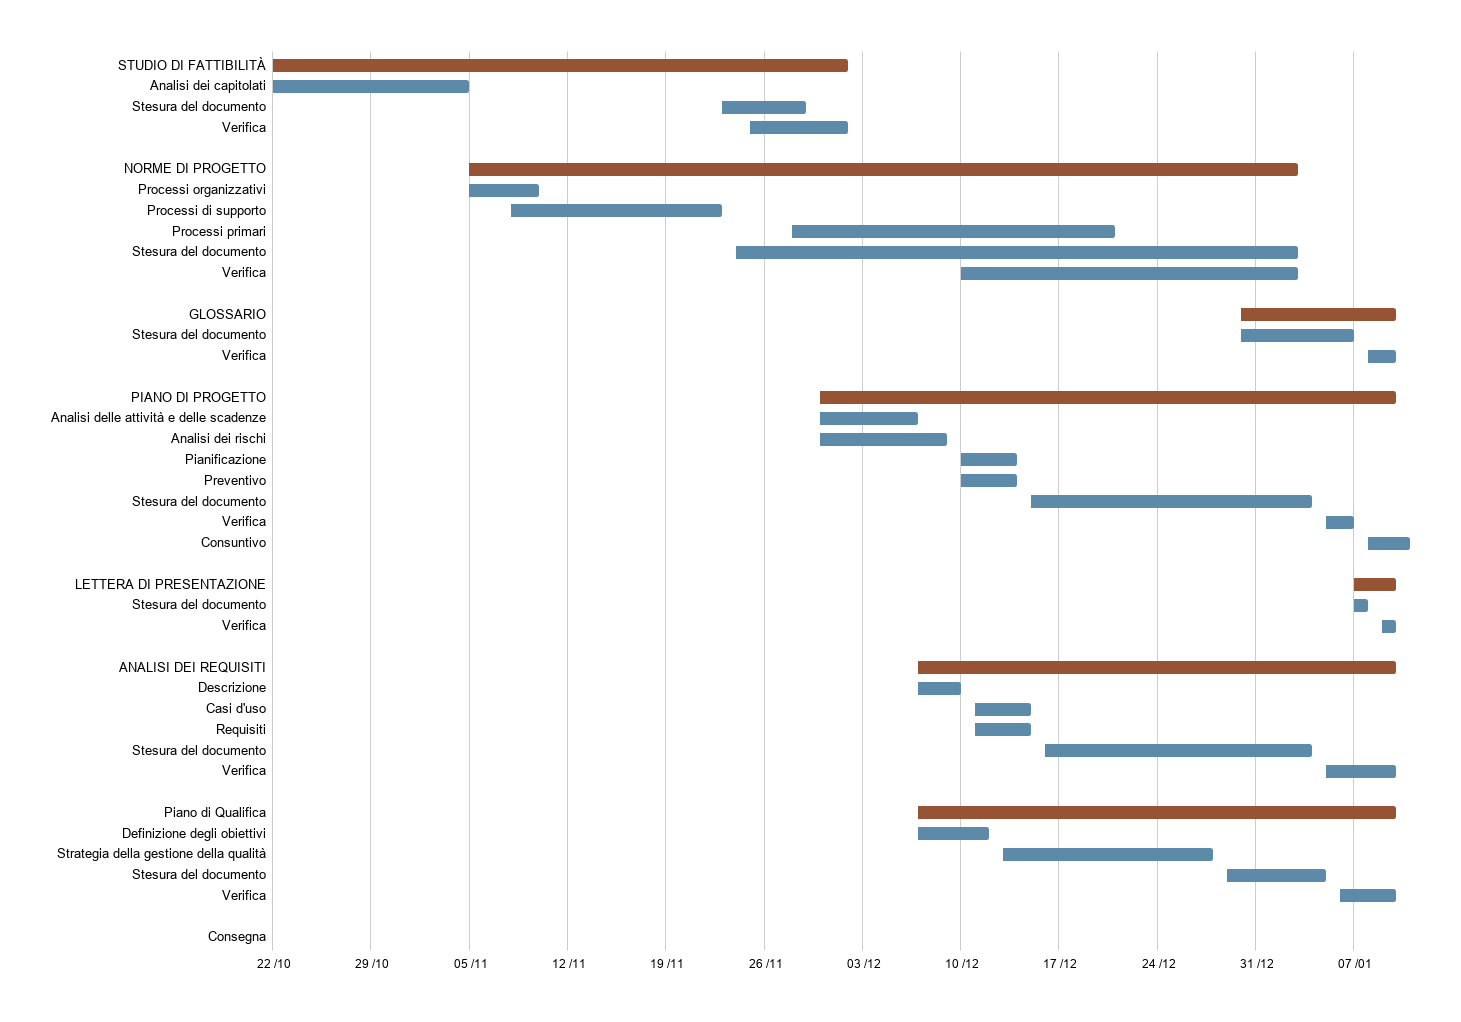
\includegraphics[width=1\linewidth]{../immagini/pdp/gantt_analisi.png}
		\caption{Diagramma di Gantt dell'attività di analisi}
	\end{center}
\end{figure}

\section{Consolidamento dei requisiti}\label{PianificazioneConsolidamentoDeiRequisiti}
\textbf{Periodo:} dal 2021-01-11 al 2021-01-18
Questo periodo ha inizio subito dopo il termine del precedente e finisce con la presentazione della Revisione dei Requisiti.
Il gruppo \textit{Jawa Druids} si dedicherà ai seguenti compiti$_{\scaleto{G}{3pt}}$:
\begin{itemize}
	\item avanzamento con lo studio individuale relativo a:
	\begin{itemize}
		\item acquisizione dei dati;
		\item simulazione dei dati;
		\item machine learning$_G$;
		\item web app.
	\end{itemize}
	\item preparazione del materiale necessario alla presentazione.
\end{itemize}
\subsection{Diagramma di Gantt: consolidamento dei requisiti}\label{PianificazioneDiagrammaDiGanttConsolidamento}
\begin{figure}[!h]
	\begin{center}
		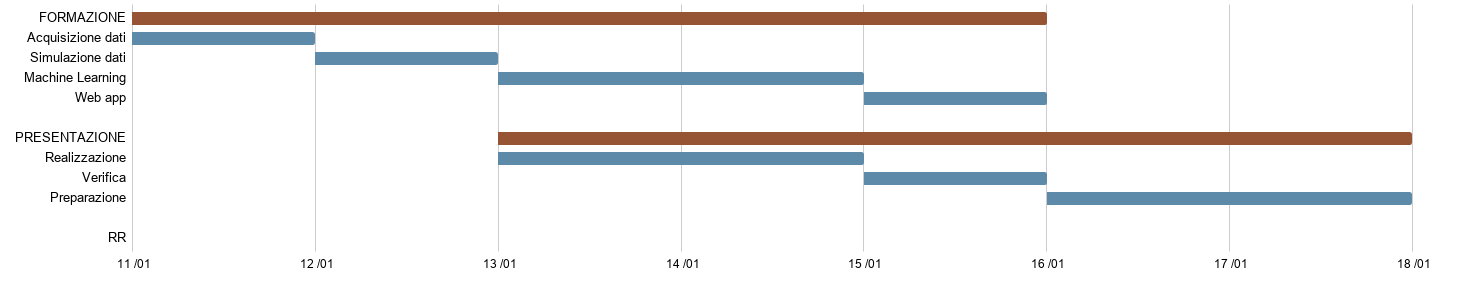
\includegraphics[width=1\linewidth]{../immagini/pdp/gantt_consolidamento_requisiti.png}
		\caption{Diagramma di Gantt del consolidamento dei requisiti}
	\end{center}
\end{figure}
\clearpage
\section{Progettazione architetturale}\label{PianificazioneProgettazioneArchitetturale}
\textbf{Periodo:} dal 2021-01-19 al 2021-03-08. \\
Questo periodo ha inizio subito dopo conclusione del precedente e termina con la Revisione di Progettazione.
Esso ha il compito di correggere ed incrementare la documentazione prodotta e di portare all'individuazione di una soluzione architetturale che permetta il soddisfacimento dei requisiti$_{\scaleto{G}{3pt}}$ obbligatori. Quindi in tale periodo si possono individuare sette incrementi nella documentazione ed una nuova attività:
\begin{itemize}
	\item \textbf{Incremento e verifica della documentazione:} analizzando l'esito della Revisione dei Requisiti, vengono svolte attività$_{\scaleto{G}{3pt}}$ di Incremento e Verifica sui vari documenti redatti, dove necessario;
	\item \textbf{Technology Baseline$_G$:}	viene realizzato un Proof of Concept$_G$ che verrà condiviso col proponente$_{\scaleto{G}{3pt}}$ per verificare il corretto sviluppo del software. In particolare il gruppo ha suddiviso ulteriormente questo incremento in due parti:
	\begin{itemize}
		\item \textbf{Prima parte} dal 2021-02-16 al 2021-02-26: in questo periodo il gruppo svilupperà 5 moduli separati, ognuno riguardante un diverso aspetto del prodotto. In particolare i moduli 1 e 2 si occuperanno di ricavare il numero di persone presenti in un determinato luogo e istante di tempo partendo dal video di una webcam, produrranno in output un dato che conterrà tale informazione. Il modulo 3 dovrà prendere in input i dati che riceve dai moduli precedenti e salvarli nel database in modo da renderli disponibili per l'utilizzo. Il modulo 4 inizierà lo sviluppo di un modello di machine learning$_{\scaleto{G}{3pt}}$ in grado di fare previsioni future. Data che questo modulo richiede una grande quantità di dati raccolti, crediamo che questa funzionalità non sarà implementata nel Proof of Concept$_{\scaleto{G}{3pt}}$. Infine il quinto modulo si occuperà di prendere gli ultimi dati caricati nel database e visualizzarli in una heat map$_{\scaleto{G}{3pt}}$.
		\item \textbf{Seconda parte} dal 2021-02-27 al 2021-03-04: nel periodo successivo il gruppo unirà tutti i prototipi dei moduli sviluppati in un unico Proof of Concept$_{\scaleto{G}{3pt}}$ che sia in grado di soddisfare alcuni dei casi d'uso$_{\scaleto{G}{3pt}}$ obbligatori. Tra questi il gruppo si pone come obiettivo che sia disponibile la heat map$_{\scaleto{G}{3pt}}$ (UC1) che prenda dati reali recentemente aggiunti al database (UC15), che vengano visualizzati i messaggi di errore in caso questi dati non siano disponibili (UC2 - UC17). Nel caso in cui ci sia la possibilità in termini di tempo, il Proof of Concept$_{\scaleto{G}{3pt}}$ continuerà ad essere sviluppato fino al termine della consegna, aggiungendo altri casi d'uso$_{\scaleto{G}{3pt}}$ obbligatori.
	\end{itemize}
\end{itemize}
\subsection{Primo Periodo}\label{PianificazioneProgettazioneArchitetturalePrimoPeriodo}
Dal 2021-01-19 al 2021-02-15: in questo primo periodo che, data la concomitanza con la sessione d'esami, risulta più esteso,  il gruppo inizierà la correzione dei documenti già redatti in concomitanza con la ricerca di fonti affidabili che ogni membro potrà consultare per fare formazione sulle tecnologie da utilizzare per la Technology Baseline$_{\scaleto{G}{3pt}}$. Inoltre saranno assegnati i vari moduli sopra citati ad ogni membro del gruppo.
\subsection{Secondo Periodo}\label{PianificazioneProgettazioneArchitetturaleSecondoPeriodo}
Dal 2021-02-16 al 2021-03-04: durante il secondo periodo il gruppo inizierà lo sviluppo del Proof of Concept$_{\scaleto{G}{3pt}}$, seguendo la divisione in due parti, quindi sviluppando prima ogni modulo separatamente e successivamente li unirà in un unico progetto. Inoltre inizierà la stesura della documentazione relativa a quest'ultimo.
\subsection{Terzo Periodo}\label{PianificazioneProgettazioneArchitetturaleTerzoPeriodo}
Dal 2021-03-05 al 2021-03-08: in questo ultimo periodo il gruppo si occuperà di verificare ogni documento e di apportare le ultime modifiche dove necessario.

\subsection{Diagramma di Gantt: progettazione architetturale}\label{PianificazioneDiagrammaDiGanttProgettazioneArchitetturale}
\begin{figure}[h]
	\begin{center}
		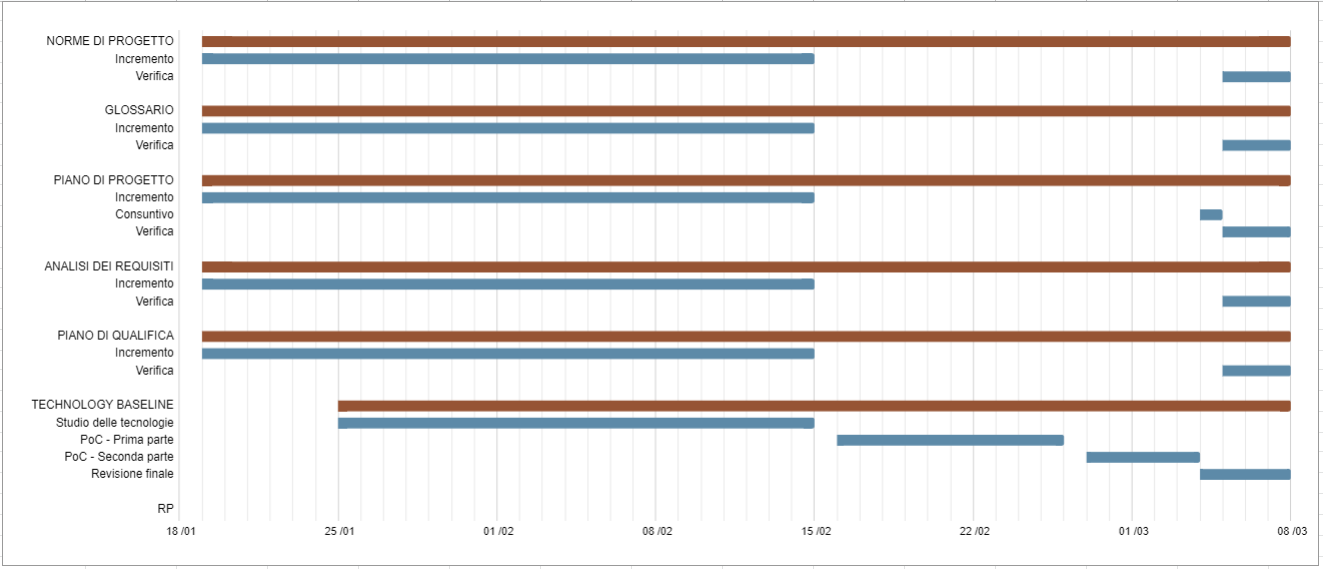
\includegraphics[width=0.9\linewidth]{../immagini/pdp/gantt_progettazione_architetturale2.png}
		\caption{Diagramma di Gantt della progettazione architetturale}
	\end{center}
\end{figure}
\clearpage
\section{Progettazione di dettaglio e codifica}\label{PianificazioneProgettazioneDettaglio}
\textbf{Periodo:} dal 2021-03-15 al 2021-04-16
Questo periodo inizia appena concluso il precedente e termina con la Revisione di Qualifica.
Le principali attività$_{\scaleto{G}{3pt}}$ svolte in questo periodo sono
\begin{itemize}
	\item \textbf{Incremento e verifica:} alcuni dei documenti già prodotti vengono migliorati e aggiornati;
	\item \textbf{Product Baseline$_G$:} segue la Technology Baseline$_{\scaleto{G}{3pt}}$, dove vengono studiati meglio design pattern$_G$, classi e attività$_{\scaleto{G}{3pt}}$ necessarie alla codifica;
	\item \textbf{Specifica Tecnica:} è un documento contenente tutte le caratteristiche del prodotto e le motivazioni che hanno portato alla loro scelta;
	\item \textbf{Codifica:} attività$_{\scaleto{G}{3pt}}$ nella quale viene prodotto e verificato il codice;
	\item \textbf{Manuale utente:} attività$_{\scaleto{G}{3pt}}$ nella quale viene redatto il documento contenente le informazioni su come funziona e su come si utilizza il prodotto.
\end{itemize}
\subsection{Periodo 1}\label{PianificazioneProgettazioneDettaglioPeriodo1}
Dal 2021-03-15 al 2021-03-22: In questo primo periodo il gruppo si dedicherà all'incremento della documentazione ed all'approfondimento delle tecnologie utilizzate per lo sviluppo del Proof of Concept$_{\scaleto{G}{3pt}}$. Partendo da quest'ultimo, inizia la fase di codifica del prodotto finale tramite il miglioramento del Proof of Concept$_{\scaleto{G}{3pt}}$ e l'ampliamento delle sue funzionalità, seguendo quanto riportato nella tabella degli incrementi della \S~\ref{ModelloDiSviluppoIncrementi}. Inizio della stesura di un manuale d'uso del prodotto destinato all'utente finale.
\subsubsection{Incrementi}\label{PianificazioneProgettazioneDettaglioPeriodo1Incrementi}
Di seguito riportiamo gli incrementi e le relative date in cui verranno svolti.
\begin{itemize}
	\item Incremento 1: dal 2021-03-15 al 2021-03-17 (3 giorni)
	\item Incremento 2: dal 2021-03-18 al 2021-03-22 (5 giorni)
\end{itemize}
\subsection{Periodo 2}\label{PianificazioneProgettazioneDettaglioPeriodo2}
Dal 2021-03-23 al 2021-04-06: seguendo quanto riportato in \S~\ref{ModelloDiSviluppoIncrementi} il gruppo si occuperà di concludere la codifica di una prima versione stabile del prodotto, implementando la maggior parte dei requisiti obbligatori e effettuerà la stesura della documentazione tecnica oltre che incrementare e correggere ulteriormente il resto della documentazione. In seguito avverrà una verifica e correzione del codice prodotto successivamente alle indicazioni ricevute in fase di Technology Baseline$_{\scaleto{G}{3pt}}$.
\subsubsection{Incrementi}\label{PianificazioneProgettazioneDettaglioPeriodo2Incrementi}
\begin{itemize}
	\item Incremento 3: dal 2021-03-23 al 2021-03-25 (3 giorni)
	\item Incremento 4: dal 2021-03-26 al 2021-03-27 (2 giorni)
	\item Incremento 5: dal 2021-03-28 al 2021-03-31 (4 giorni)
	\item Incremento 6: dal 2021-04-01 al 2021-04-01 (1 giorno)
	\item Incremento 7: dal 2021-04-02 al 2021-04-03 (2 giorni)
	\item Incremento 8: dal 2021-04-04 al 2021-04-05 (2 giorni)
	\item Incremento 9: dal 2021-04-06 al 2021-04-07 (2 giorni)
\end{itemize}
\subsection{Periodo 3}\label{PianificazioneProgettazioneDettaglioPeriodo3}
Dal 2021-04-07 al 2021-04-16: nel periodo finale di questa fase il gruppo si occuperà del completamento del manuale d'uso per l'utente. In seguito verranno conclusi i documenti per la consegna della Revisione di Qualifica ed il gruppo si preparerà all'esposizione.
\subsubsection{Incrementi}\label{PianificazioneProgettazioneDettaglioPeriodo3Incrementi}
\begin{itemize}
	\item Incremento 10: dal 2021-04-07 al 2021-04-09 (3 giorni)
	\item Incremento 11: dal 2021-04-10 al 2021-04-16 (7 giorni)
\end{itemize}
\clearpage
\subsection{Diagramma di Gantt: progettazione di dettaglio e codifica}\label{PianificazioneDiagrammaDiGanttProgettazioneDettaglio}
\begin{figure}[!h]
	\begin{center}
		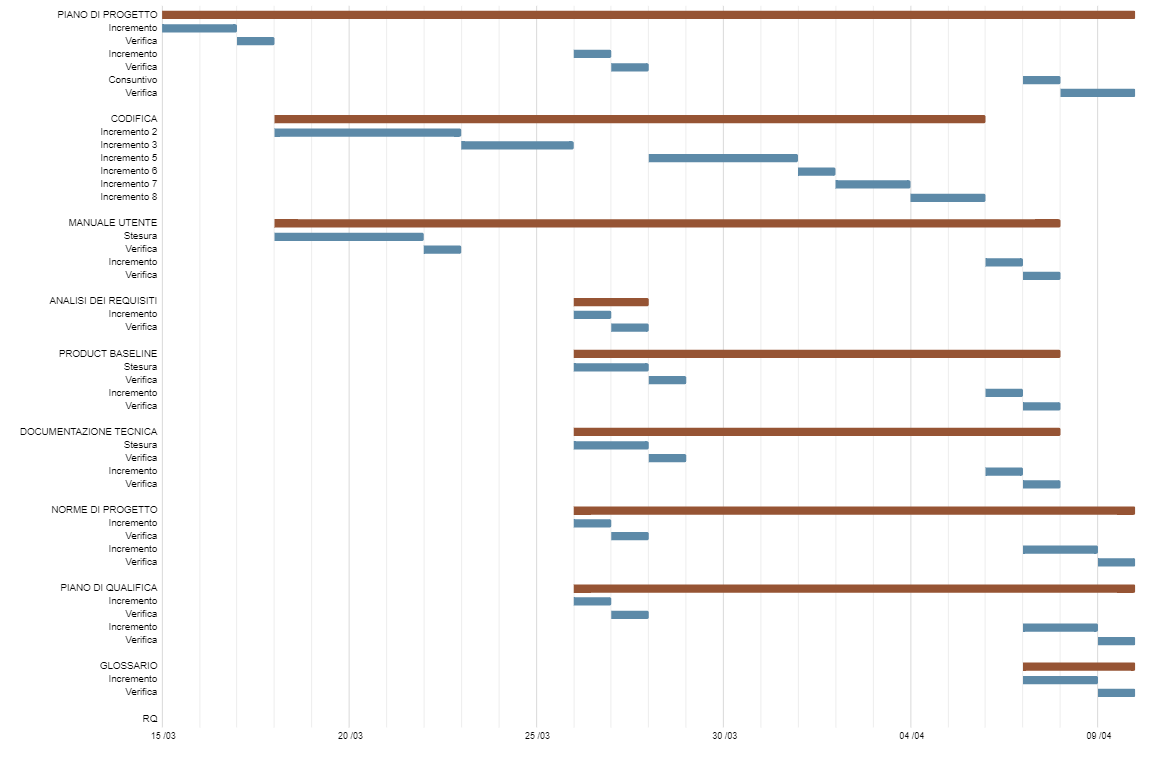
\includegraphics[width=1\linewidth]{../immagini/pdp/gantt_progettazione_dettaglio3.png}
		\caption{Diagramma di Gantt dell'attività di progettazione di dettaglio e codifica}
	\end{center}
\end{figure}





\clearpage
\section{Validazione e Collaudo}\label{PianificazioneValidazioneCollaudo}
\textbf{Periodo:} dal 2021-04-30 al 2021-05-23
Questo periodo inizia appena concluso il precedente e termina con la Revisione di Accettazione.\\

Le principali attività$_{\scaleto{G}{3pt}}$ svolte in questo periodo sono:
\begin{itemize}
	\item \textbf{Incremento e verifica dei documenti:} analizzando l'esito della Revisione di Qualifica vengono svolte attività$_{\scaleto{G}{3pt}}$ di Incremento e Verifica sui vari documenti redatti;
	\item \textbf{Codifica:} attività$_{\scaleto{G}{3pt}}$ nella quale viene prodotto e verificato il codice legato a eventuali requisiti opzionali e modifiche per garantire stabilità e sicurezza;
	\item \textbf{Validazione e Collaudo:} vengono realizzati i Test di Sistema e Test di Accettazione, con i dovuti controlli finali, in modo da garantire un buon livello di qualità e correttezza.
\end{itemize}

La pianificazione di questo periodo ha subito importanti modifiche a causa dei consuntivi dei periodi precedenti: dato l'eccesso di risorse utilizzate nelle fasi di \textit{Progettazione architetturale} e \textit{Progettazione di dettaglio e codifica}, il gruppo ha deciso di allocare meno ore di lavoro e risorse per rientrare nei costi previsti dal preventivo.
La stima di risorse per le attività di Codifica, Validazione e Collaudo hanno subito considerevoli riduzioni e modifiche, a causa del buon livello di codifica e verifica ottenuto nelle fasi precedenti e l'inizio dello stage da parte di alcuni partecipanti; inoltre anche la stima di risorse per l'attività di Incremento e Verifica dei documenti ha subito delle riduzioni dato il minor numero di modifiche necessarie conseguenti alla Revisione di Qualifica.

L'obiettivo è quello di rientrare nel costo per l'intero progetto inizialmente preventivato di 14.480\euro; per ottenere questo risultato il gruppo pianifica una riduzione dal numero di ore totali per questa fase da 175 (preventivate inizialmente) a 91(-84), e una riduzione del costo che passa da 3080\euro (preventivato inizialmente) a 1605\euro(-1475\euro).
Il gruppo ritiene che il taglio di risorse in questa fase non implichi alcuna diminuzione di qualità del prodotto finale, poiché queste riduzioni sono una conseguenza del buono stato di avanzamento delle fasi precedenti.  \\
Ogni incremento prevede anche la sua verifica. \\

% \subsection{Periodo 1}
% Dal 2021-04-30 al 2021-05-05: in questo periodo il gruppo implementerà alcuni dei requisiti facoltativi e desiderabili e si occuperà di aggiornare il manuale utente e la documentazione tecnica in base alle modifiche effettuate.
\subsection{Incrementi pianificati}
\begin{itemize}
	\item \textbf{Incremento 12:}
	Implementazione di eventuali requisiti facoltativi e desiderabili tra quelli elencati nell'\textit{Analisi dei Requisiti v4.0.0}. \\
	Stima delle risorse:
  \begin{itemize}
		\item \textbf{Intervallo temporale:} 3 giorni (dal 2021-04-30 al 2021-05-02);
		\item \textbf{Prospetto orario:} 2 ore AM, 9 ore PR, 3 ore VE;
		\item \textbf{Costo pianificato:} 220\euro.
	\end{itemize}
	Il gruppo pianifica di soffisdare i seguenti requisiti facoltativi:
		\begin{itemize}
			\item RSFD34;
			\item RSFF31;
			\item RSFD33.2.
		\end{itemize}

	\item \textbf{Incremento 13}:
	Incremento e revisione finale del Manuale Utente.\\
	Stima delle risorse:
  \begin{itemize}
		\item \textbf{Intervallo temporale:} 1 giorno (dal 2021-05-03 al 2021-05-03);
		\item \textbf{Prospetto orario:} 1 ore RE, 3 ore PR, 4 ore VE;
		\item \textbf{Costo pianificato:} 135\euro.
	\end{itemize}

	\item \textbf{Incremento 14}:
	Incremento della documentazione tecnica.\\
	Stima delle risorse:
	\begin{itemize}
		\item \textbf{Intervallo temporale:} 2 giorni (dal 2021-05-04 al 2021-05-05);
		\item \textbf{Prospetto orario:} 1 ore RE, 5 ore PR, 5 ore VE;
		\item \textbf{Costo pianificato:} 180\euro.
	\end{itemize}
% \end{itemize}
% \subsection{Periodo 2}
% Dal 2021-05-06 al 2021-05-15: nel secondo periodo il gruppo si occuperà della correzione della codifica e della documentazione in base ad eventuali indicazioni ricevute in fase di Revisione di Qualifica.
% \subsection{Incrementi}
% \begin{itemize}
\item \textbf{Incremento 15}:
Correzione e revisione della codifica.\\
Stima delle risorse:
\begin{itemize}
	\item \textbf{Intervallo temporale:} 5 giorni (dal 2021-05-06 al 2021-05-10);
	\item \textbf{Prospetto orario:} 7 ore VE;
	\item \textbf{Costo pianificato:} 105\euro.
\end{itemize}

\item \textbf{Incremento 16}:
Incremento e correzione della documentazione in base alle indicazioni ricevute in Revisione di Qualifica.\\
\textbf{Incremento 16.1}
Incremento e correzione del Piano di Progetto.\\
Stima delle risorse:
\begin{itemize}
	\item \textbf{Intervallo temporale:} 3 giorni (dal 2021-05-11 al 2021-05-13);
	\item \textbf{Prospetto orario:} 6 ore RE, 4 ore VE;
	\item \textbf{Costo pianificato:} 240\euro.
\end{itemize}
\textbf{Incremento 16.2}
Incremento e correzione del Piano di Qualifica.\\
Stima delle risorse:
\begin{itemize}
	\item \textbf{Intervallo temporale:} 1 giorno (dal 2021-05-14 al 2021-05-14);
	\item \textbf{Prospetto orario:} 1 ore RE, 3 ore AM, 6 ore VE;
	\item \textbf{Costo pianificato:} 180\euro.
\end{itemize}
\textbf{Incremento 16.3}
Incremento e correzione del Glossario.\\
Stima delle risorse:
\begin{itemize}
	\item \textbf{Intervallo temporale:} 1 giorno (dal 2021-05-15 al 2021-05-15);
	\item \textbf{Prospetto orario:} 1 ore RE, 3 ore VE;
	\item \textbf{Costo pianificato:} 75\euro.
\end{itemize}

	% \item Incremento 16: dal 2021-05-11 al 2021-05-15 (5 giorni)
% \end{itemize}
% \subsection{Periodo 3}
% Dal 2021-05-16 al 2021-05-23: validazione e collaudo del prodotto per consegna in Revisione di Accettazione.
% \subsubsection{Incrementi}
% \begin{itemize}

\item \textbf{Incremento 17}:
Validazione del software e documentazione prodotta.\\
Stima delle risorse:
\begin{itemize}
	\item \textbf{Intervallo temporale:} 4 giorni (dal 2021-05-16 al 2021-05-19);
	\item \textbf{Prospetto orario:} 2 ore RE, 2 ore AM, 9 ore VE;
	\item \textbf{Costo pianificato:} 235\euro.
\end{itemize}

\item \textbf{Incremento 18}:
Collaudo del software.\\
Stima delle risorse:
\begin{itemize}
	\item \textbf{Intervallo temporale:} 4 giorni (dal 2021-05-20 al 2021-05-23);
	\item \textbf{Prospetto orario:} 1 ore RE, 2 ore AM, 11 ore VE;
	\item \textbf{Costo pianificato:} 235\euro.
\end{itemize}

\end{itemize}

\clearpage
\subsection{Consumo delle risorse pianificato per la fase di Validazione e collaudo}

Nella seguente tabella riassumiamo il consumo di risorse pianificato per la fase di Validazione e collaudo, con le differenze rispetto al preventivo per questa fase.

\quad
\def\tabularxcolumn#1{m{#1}}
{\rowcolors{2}{RawSienna!90!RawSienna!20}{RawSienna!70!RawSienna!40}

	\begin{center}
		\renewcommand{\arraystretch}{1.4}
		\begin{tabularx}{\textwidth}{|X|c|c|c|c|c|c|c|c|}
			\hline
			\rowcolor{airforceblue}
			\textbf{Incremento} & \textbf{Re} & \textbf{Am} & \textbf{An} & \textbf{Pt} & \textbf{Pr} & \textbf{Ve} & \textbf{Ore totali} & \textbf{Costo} \\
			\hline
			\textit{Incremento 12} & 0(-2) & 2(-1) & 0 & 0 & 9(-5) & 3(+3) & 14(-5) & 220\euro(-110\euro) \\
			\hline
			\textit{Incremento 13} & 1 & 0(-2) & 0 & 0 & 3(+3) & 4(-6) & 8(-5) & 135\euro(-85\euro) \\
			\hline
			\textit{Incremento 14} & 1(-1) & 0(-3) & 0 & 0 & 5(+5) & 5(-8) & 11(-7) & 180\euro(-135\euro) \\
			\textit{Incremento 15} & 0(-3) & 0(-7) & 0 & 0 & 0(-24) & 7(+7) & 7(-27) & 105\euro(-485\euro) \\
			\textit{Incremento 16} & 8 & 3(-3) & 0 & 0 & 0 & 13(-24) & 24(-27) & 495\euro(-420\euro) \\
			\textit{Incremento 17} & 2(-1) & 2 & 0 & 0 & 0(-14) & 9(+9) & 13(-6) & 235\euro(-105\euro) \\
			\hline
			\textit{Incremento 18} & 1(-1) & 2(-3) & 0 & 0 & 0(-14) & 11(+11) & 14(-7) & 235\euro(-135\euro) \\
			\hline
			\textbf{Totale} & 13(-8) & 9(-19) & 0 & 0 & 17(-49) & 52(-8) & 91(-84) & 1605\euro(-1475\euro) \\
			\hline
		\end{tabularx}
			\captionof{table}{\textbf{Consumo delle risorse pianificato per la fase di Validazione e collaudo}}
	\end{center}

	% \item Incremento 17: dal 2021-05-16 al 2021-05-19 (4 giorni)
	% \item Incremento 18: dal 2021-05-20 al 2021-05-23 (4 giorni)
\clearpage
\subsection{Diagramma di Gantt: validazione e collaudo}\label{PianificazioneDiagrammaDiGanttValidazione}
\begin{figure}[!h]
	\begin{center}
		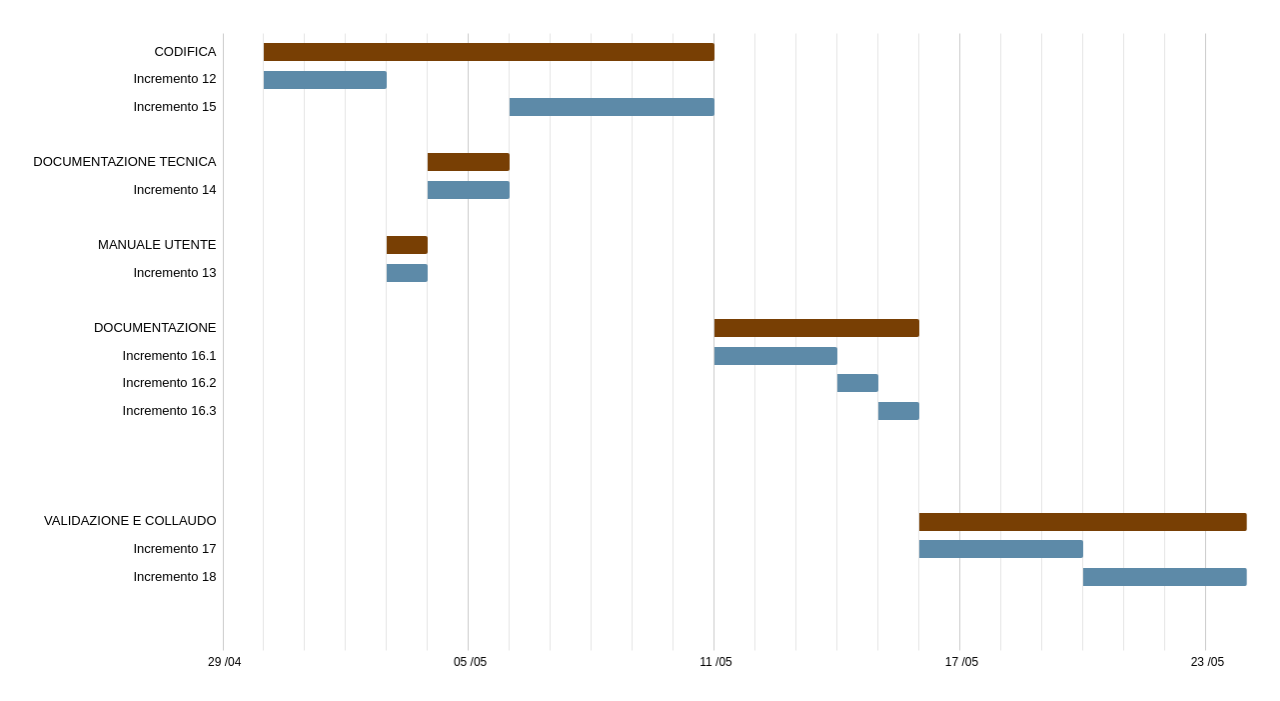
\includegraphics[width=1\linewidth]{../immagini/pdp/gantt_validazione_updated.png}
		\caption{Diagramma di Gantt dell'attività di validazione e collaudo}
	\end{center}
\end{figure}
